\documentclass[aspectratio=169,11pt]{beamer}
\usepackage[T1]{fontenc}
\usepackage{lmodern,amsmath,amssymb,mathtools,bm,booktabs,array,graphicx,tikz}
\usetikzlibrary{arrows.meta,positioning,calc,decorations.pathreplacing,patterns}
\definecolor{ink}{HTML}{17344D}\definecolor{accent}{HTML}{087E8B}\definecolor{pale}{HTML}{EDF5F5}\definecolor{gold}{HTML}{AD6B19}
\providecommand{\dd}{\,\mathrm{d}}\providecommand{\R}{\mathbb{R}}
\providecommand{\E}{\mathbb{E}}\providecommand{\Var}{\operatorname{Var}}
\providecommand{\Cov}{\operatorname{Cov}}\providecommand{\diag}{\operatorname{diag}}
\providecommand{\norm}[1]{\left\lVert#1\right\rVert}
\providecommand{\abs}[1]{\left|#1\right|}
\usefonttheme{professionalfonts}
\setbeamercolor{normal text}{fg=black,bg=white}
\setbeamercolor{frametitle}{fg=ink,bg=white}
\setbeamercolor{title}{fg=ink}\setbeamercolor{structure}{fg=accent}
\setbeamercolor{block title}{fg=ink,bg=pale}\setbeamercolor{block body}{fg=black,bg=pale!40}
\setbeamercolor{alerted text}{fg=accent}
\setbeamerfont{frametitle}{size=\Large,series=\bfseries}
\setbeamerfont{title}{size=\LARGE,series=\bfseries}
\setbeamertemplate{navigation symbols}{}
\setbeamersize{text margin left=.7cm,text margin right=.7cm}
\setbeamertemplate{frametitle}{\vspace{.18cm}\insertframetitle\par\vspace{.1cm}{\color{accent}\hrule height .6pt}\vspace{.12cm}}
\newcommand{\notestarget}{notes.pdf}\newcommand{\noteslabel}{Notes}
\setbeamertemplate{footline}{\hspace{.7cm}\color{ink}\scriptsize Computational Cardiology\quad\href{\notestarget}{\noteslabel}\hfill\insertframenumber\,/\,\inserttotalframenumber\hspace{.7cm}\vspace{.18cm}}
\setbeamercovered{invisible}
\hypersetup{pdfauthor={Zan Ahmad},pdftitle={Spectral attenuation surrogates and graph-basis limitations},pdfpagemode=UseNone}
\begin{document}
\begin{frame}[plain]\vfill
{\small\color{accent} Computational Cardiology \quad Lecture 18}\par\medskip
{\raggedright\hyphenpenalty=10000\exhyphenpenalty=10000\LARGE\bfseries\color{ink} Spectral attenuation surrogates and graph-basis limitations}\par\bigskip
Zan Ahmad\par\smallskip
{\small Fall 2024}\par\vfill\end{frame}
\renewcommand{\notestarget}{notes.pdf\#note-the-research-operator-and-the-finite-baseline}
\begin{frame}[t,fragile,label=slide-a-three-parameter-fixed-time-map]{A three-parameter fixed-time map}
\[\widehat\Phi_T[u]=a_0+\sum_{k=1}^3q_k a_k\cos(k\pi x/L).\]\pause{} The mean passes through unchanged; three gains are fitted.
\end{frame}
\renewcommand{\notestarget}{notes.pdf\#note-projection-inner-products-and-null-modes}
\begin{frame}[t,fragile,label=slide-resolved-midpoint-projection]{Resolved midpoint projection}
\[a_0=\frac1N\sum_i u_i,\qquad a_k=\frac2N\sum_i u_i\cos(k\pi x_i/L).\]\pause{} Exact coefficient recovery here relies on the resolved finite cosine family.
\end{frame}
\renewcommand{\notestarget}{notes.pdf\#note-projection-inner-products-and-null-modes}
\begin{frame}[t,fragile,label=slide-projection-and-reconstruction]{Projection and reconstruction}
\[u\longmapsto(a_0,a_1,a_2,a_3)\longmapsto(a_0,q_1a_1,q_2a_2,q_3a_3)\longmapsto\widehat u.\]\pause{} Omitted input modes cannot reappear through this diagonal map.
\end{frame}
\renewcommand{\notestarget}{notes.pdf\#note-projection-inner-products-and-null-modes}
\begin{frame}[t,fragile,label=slide-a-graph-normalized-laplacian]{A graph-normalized Laplacian}
\[L_{sym}=I-D^{-1/2}WD^{-1/2}.\]\pause{} Assume positive degrees. Its eigenvectors use the Euclidean inner product of the normalized representation.
\end{frame}
\renewcommand{\notestarget}{notes.pdf\#note-projection-inner-products-and-null-modes}
\begin{frame}[t,fragile,label=slide-the-normalized-null-mode]{The normalized null mode}
\[L_{sym}D^{1/2}\boldsymbol1=0.\]\pause{} The zero mode is proportional to square-root degree, generally not the constant vector.
\end{frame}
\renewcommand{\notestarget}{notes.pdf\#note-least-squares-identification-of-modal-gains}
\begin{frame}[t,fragile,label=slide-least-squares-for-one-gain]{Least squares for one gain}
\[J(q)=\sum_j(b_j-qa_j)^2.\]\pause{}\[J^{\prime}(q)=-2\sum_ja_jb_j+2q\sum_ja_j^2.\]
\end{frame}
\renewcommand{\notestarget}{notes.pdf\#note-least-squares-identification-of-modal-gains}
\begin{frame}[label=slide-the-fitted-attenuation-panel-1]{An exactly representable fit}
\centering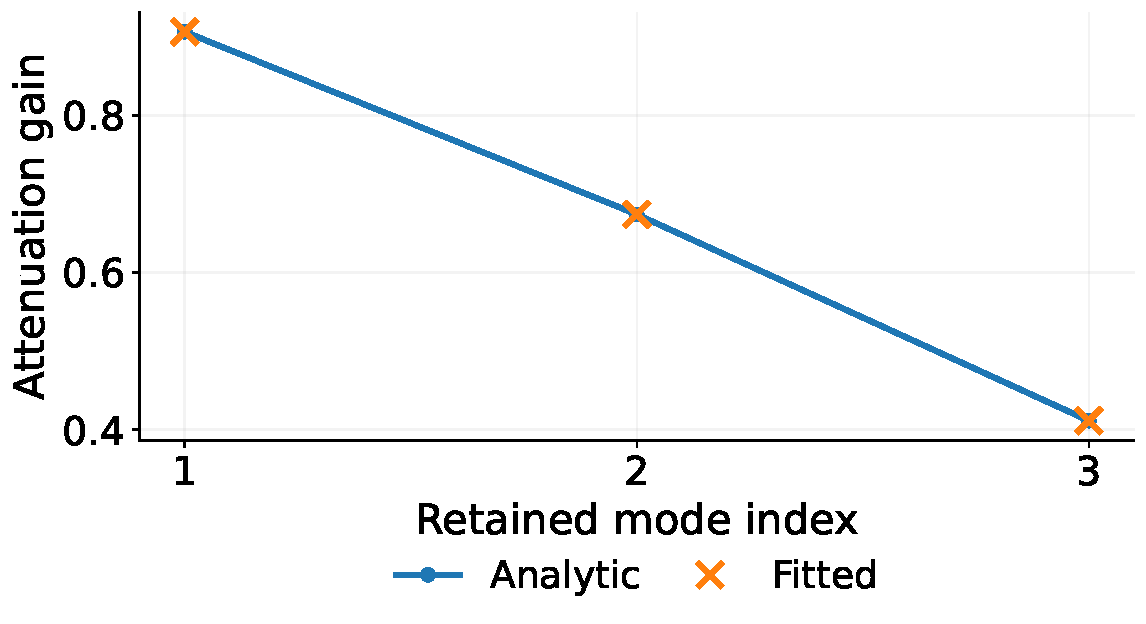
\includegraphics[width=.98\linewidth,height=.69\textheight,keepaspectratio]{presentation-figures/spectral-baseline-panel-1.pdf}\end{frame}
\renewcommand{\notestarget}{notes.pdf\#note-least-squares-identification-of-modal-gains}
\begin{frame}[label=slide-the-fitted-attenuation-panel-2]{Reuse on a finer sampling grid}
\centering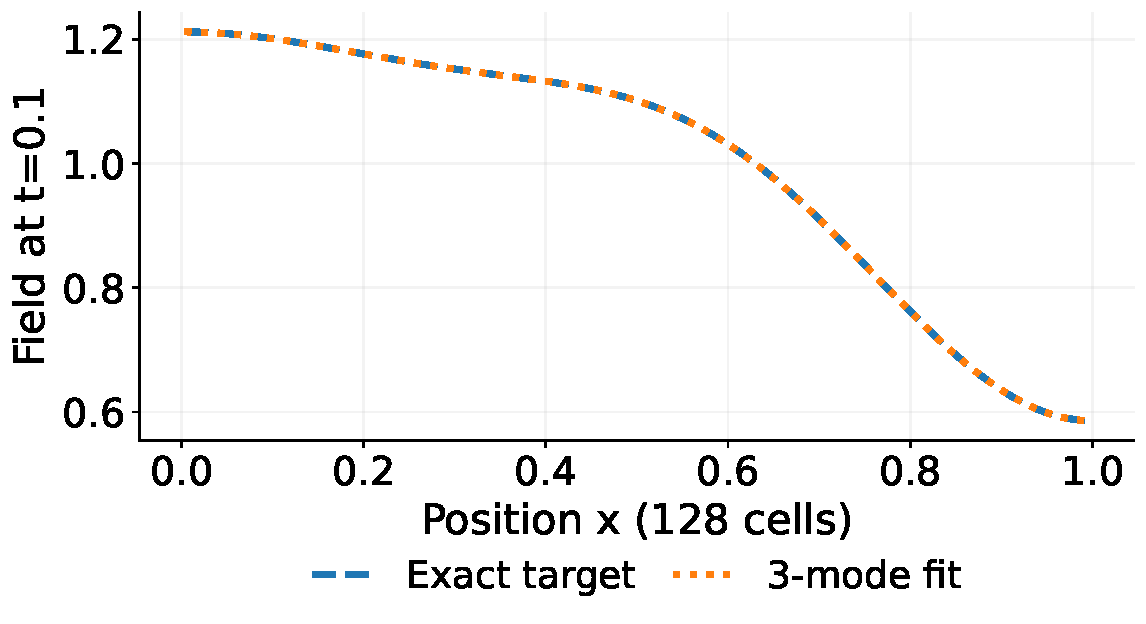
\includegraphics[width=.98\linewidth,height=.69\textheight,keepaspectratio]{presentation-figures/spectral-baseline-panel-2.pdf}\end{frame}
\renewcommand{\notestarget}{notes.pdf\#note-least-squares-identification-of-modal-gains}
\begin{frame}[t,fragile,label=slide-the-fitted-attenuation]{The fitted attenuation}
\[\widehat q=\frac{\sum_ja_jb_j}{\sum_ja_j^2}.\]\pause{} A positive denominator gives a unique minimizer.
\end{frame}
\renewcommand{\notestarget}{notes.pdf\#note-least-squares-identification-of-modal-gains}
\begin{frame}[t,fragile,label=slide-an-unexcited-mode-is-unidentified]{An unexcited mode is unidentified}
If $a_j=0$ for every case, $J(q)=\sum_jb_j^2$ for every $q$.\pause{} No optimizer can recover a gain from absent excitation.
\end{frame}
\renewcommand{\notestarget}{notes.pdf\#note-least-squares-identification-of-modal-gains}
\begin{frame}[t,fragile,label=slide-exact-representability-explains-the-fit]{Exact representability explains the fit}
\[q_k=e^{-\kappa(k\pi/L)^2T}.\]\pause{} Noiseless exact labels, a known basis and three excited modes make near-roundoff error expected in the stated family.
\end{frame}
\renewcommand{\notestarget}{notes.pdf\#note-resolved-grid-reuse-and-omitted-input-modes}
\begin{frame}[t,fragile,label=slide-reuse-on-another-resolved-grid]{Reuse on another resolved grid}
The same continuous coefficients are projected and reconstructed on a new midpoint grid.\pause{} This changes sampling density while retaining the domain, bandwidth, diffusivity and time.
\end{frame}
\renewcommand{\notestarget}{notes.pdf\#note-resolved-grid-reuse-and-omitted-input-modes}
\begin{frame}[label=slide-an-omitted-fourth-mode-panel-1]{Changed diffusivity}
\centering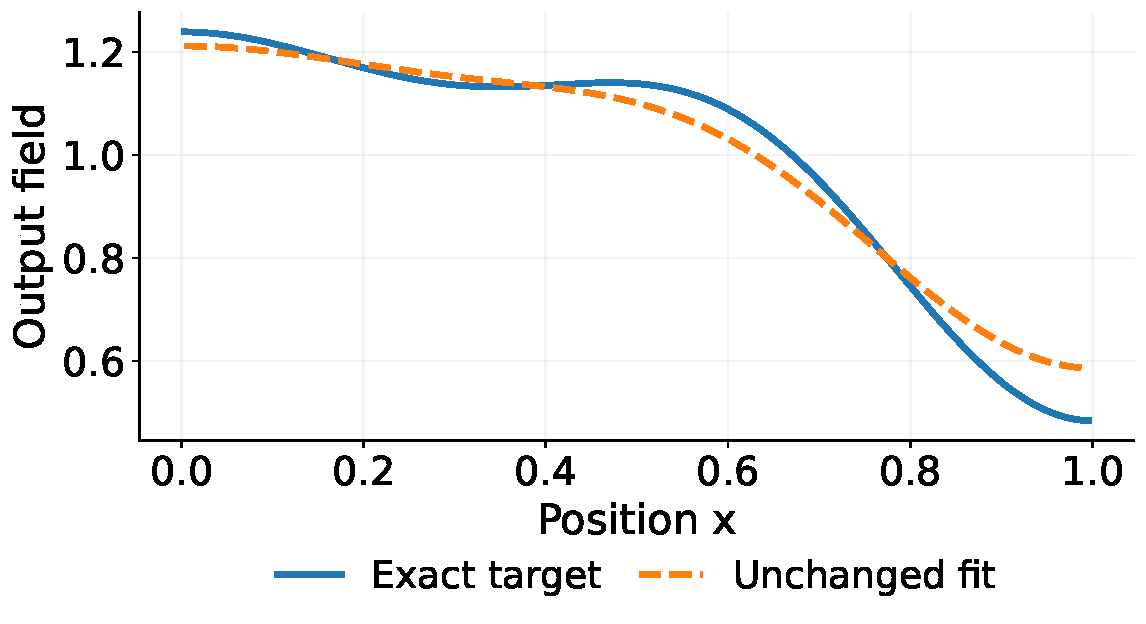
\includegraphics[width=.98\linewidth,height=.69\textheight,keepaspectratio]{presentation-figures/transfer-failures-panel-1.pdf}\end{frame}
\renewcommand{\notestarget}{notes.pdf\#note-resolved-grid-reuse-and-omitted-input-modes}
\begin{frame}[label=slide-an-omitted-fourth-mode-panel-2]{An omitted input mode}
\centering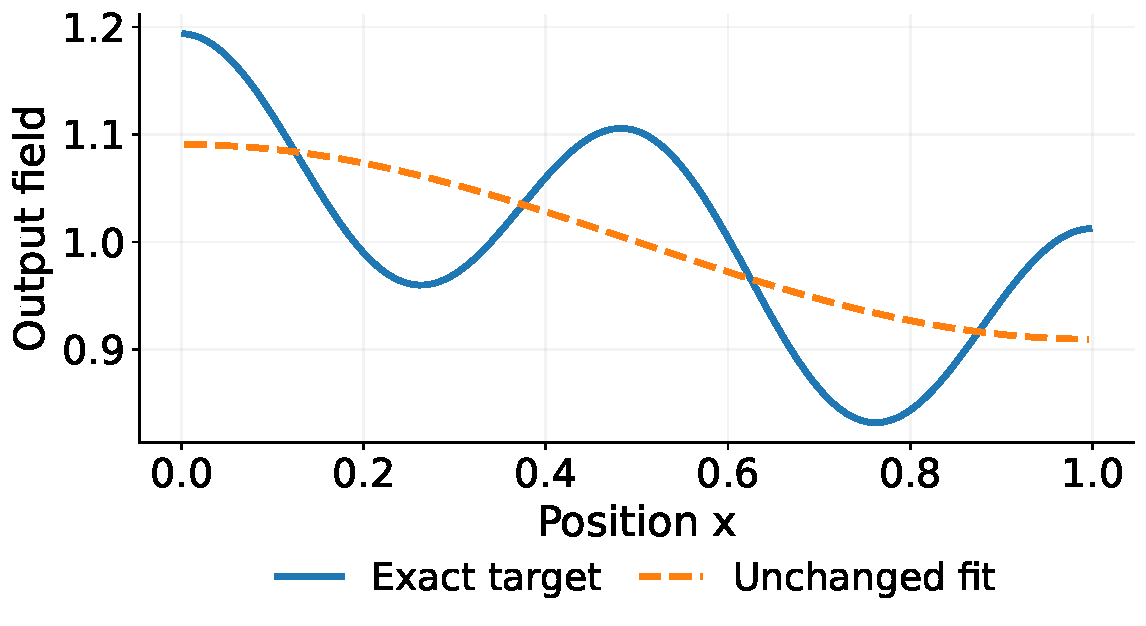
\includegraphics[width=.98\linewidth,height=.69\textheight,keepaspectratio]{presentation-figures/transfer-failures-panel-2.pdf}\end{frame}
\renewcommand{\notestarget}{notes.pdf\#note-resolved-grid-reuse-and-omitted-input-modes}
\begin{frame}[t,fragile,label=slide-an-omitted-fourth-mode]{An omitted fourth mode}
\[E_{RMS}=\frac{|a_4|}{\sqrt2}e^{-\kappa(4\pi/L)^2T}.\]\pause{} The mean can remain exact while this nonconstant output is missing.
\end{frame}
\renewcommand{\notestarget}{notes.pdf\#note-resolved-grid-reuse-and-omitted-input-modes}
\begin{frame}[t,fragile,label=slide-a-changed-diffusivity]{A changed diffusivity}
\[e^{-\kappa_{train}(k\pi/L)^2T}\ne e^{-\kappa_{test}(k\pi/L)^2T}.\]\pause{} Keeping the basis does not correct gains fitted for another operator.
\end{frame}
\renewcommand{\notestarget}{notes.pdf\#note-basis-changes-and-spectral-consistency}
\begin{frame}[t,fragile,label=slide-consistent-eigenvector-sign-changes]{Consistent eigenvector sign changes}
\[K=\Phi Q\Phi^{\mathsf T}=(\Phi S)Q(\Phi S)^{\mathsf T},\qquad S^2=I.\]\pause{} Diagonal gains commute with sign flips.
\end{frame}
\renewcommand{\notestarget}{notes.pdf\#note-basis-changes-and-spectral-consistency}
\begin{frame}[t,fragile,label=slide-repeated-eigenspaces-require-more]{Repeated eigenspaces require more}
\[Q\longmapsto OQO^{\mathsf T}.\]\pause{} Invariance to every orthogonal change within a block requires identical gains on that block.
\end{frame}
\renewcommand{\notestarget}{notes.pdf\#note-fixed-time-maps-and-learned-generators}
\begin{frame}[t,fragile,label=slide-the-research-scope-remains-broader]{The research scope remains broader}
GFuNK learns graph-spectral nonlinear generators and integrates trajectories across specified geometry and diffusion families.\pause{} The three-gain companion is a fixed-time baseline, not that architecture.
\end{frame}
\end{document}
